\documentclass{article}

\usepackage[spanish]{babel}
\usepackage[numbers,sort&compress]{natbib}
\usepackage[T1]{fontenc}
\usepackage[ansinew]{inputenc}
\usepackage{graphicx}
\usepackage{url}
\usepackage{caption}
\usepackage{float}

\title {Sistema Multiagente}
\author{Oscar Qui\~nonez}

\begin{document}

\maketitle
 
\section{Objetivo}\label{met}

Para realizar el proyecto 6, se implementa un sistema multiagente \cite{satuelisa}, en el que se simula el contagio entre un grupo de personas que tienen contacto entre ellas, se busca entonces determinar la probabilidad de contagio de las personas vacunadas y la manera en la que se propagar\'ia el contagio entre las no vacunadas.

\section{Metodolog\'ia}\label{met}

En esta simulaci\'on se requiri\'o del uso del programa R 4.0.2, tomando como base el c\'odigo \cite{satu} para la modificaci\'on en cuanto al n\'umero de agentes, dado que pv representa a la parte de la muestra que ya hab\'ia sido vacunada previamente y por lo tanto no se contagian ni pueden contagiar a los dem\'as miembros de la muestra total. Los datos m\'as relevantes, y por lo tanto mas importantes para nosotros son el porcentaje m\'aximo de contagio que puede haber en la muestra y el momento en el que esto ocurre.

\section{Resultados y Discusi\'on}\label{res}

Al variar el valor de pv entre 0 y 1 con pasos de 0.1 se muestra un cambio en el comportamiento de los infectados, pues recordemos que algunos ya estaban vacunados pero la mayor\'ia segu\'ian sin estarlo y por lo tanto eran mas vulnerables a contraer el contagio y transmitirlo entre el resto de la muestra que tampoco hab\'ia sido vacunada con anterioridad. El porcentaje m\'aximo se ve representado en la figura 1 en la que cada barra representa una variaci\'on de 0.1 entre los valores de 0 y 1, es decir que cada una es un avance del 10\%; por lo tanto, se puede apreciar que mientras mayor sea la cantidad de vacunados, menor es la probabilidad de contagio entre el grupo y as\'i se ve reflejada la efectividad que lleva para la poblaci\'on total que todos o casi todos est\'en vacunados.

\begin{figure}
  \centering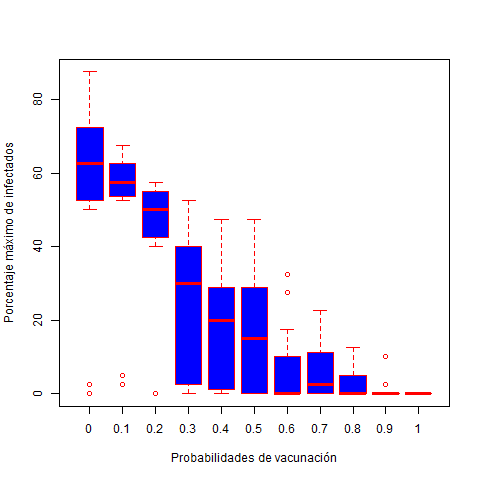
\includegraphics[scale=0.7]{tareaseisboxplot.png}
  \caption{Variaci\'on en la probalilidad de vacunaci\'on.}
  \label{fig}
\end{figure}

\newpage
En la figura 2 mostrada anteriormente nos indica que el porcentaje m\'aximo de contagios es de 87.5\% de los 40 agentes estudiados, que equivalen a 35 de ellos, adem\'as de que tambi\'en se muestra una disminuci\'on mientras van aumentando los vacunados. Los datos tambi\'en se muestran en la tabla 1 obtenida del archivo de texto generado por el c\'odigo \cite{yo}.

\begin{figure}
  \centering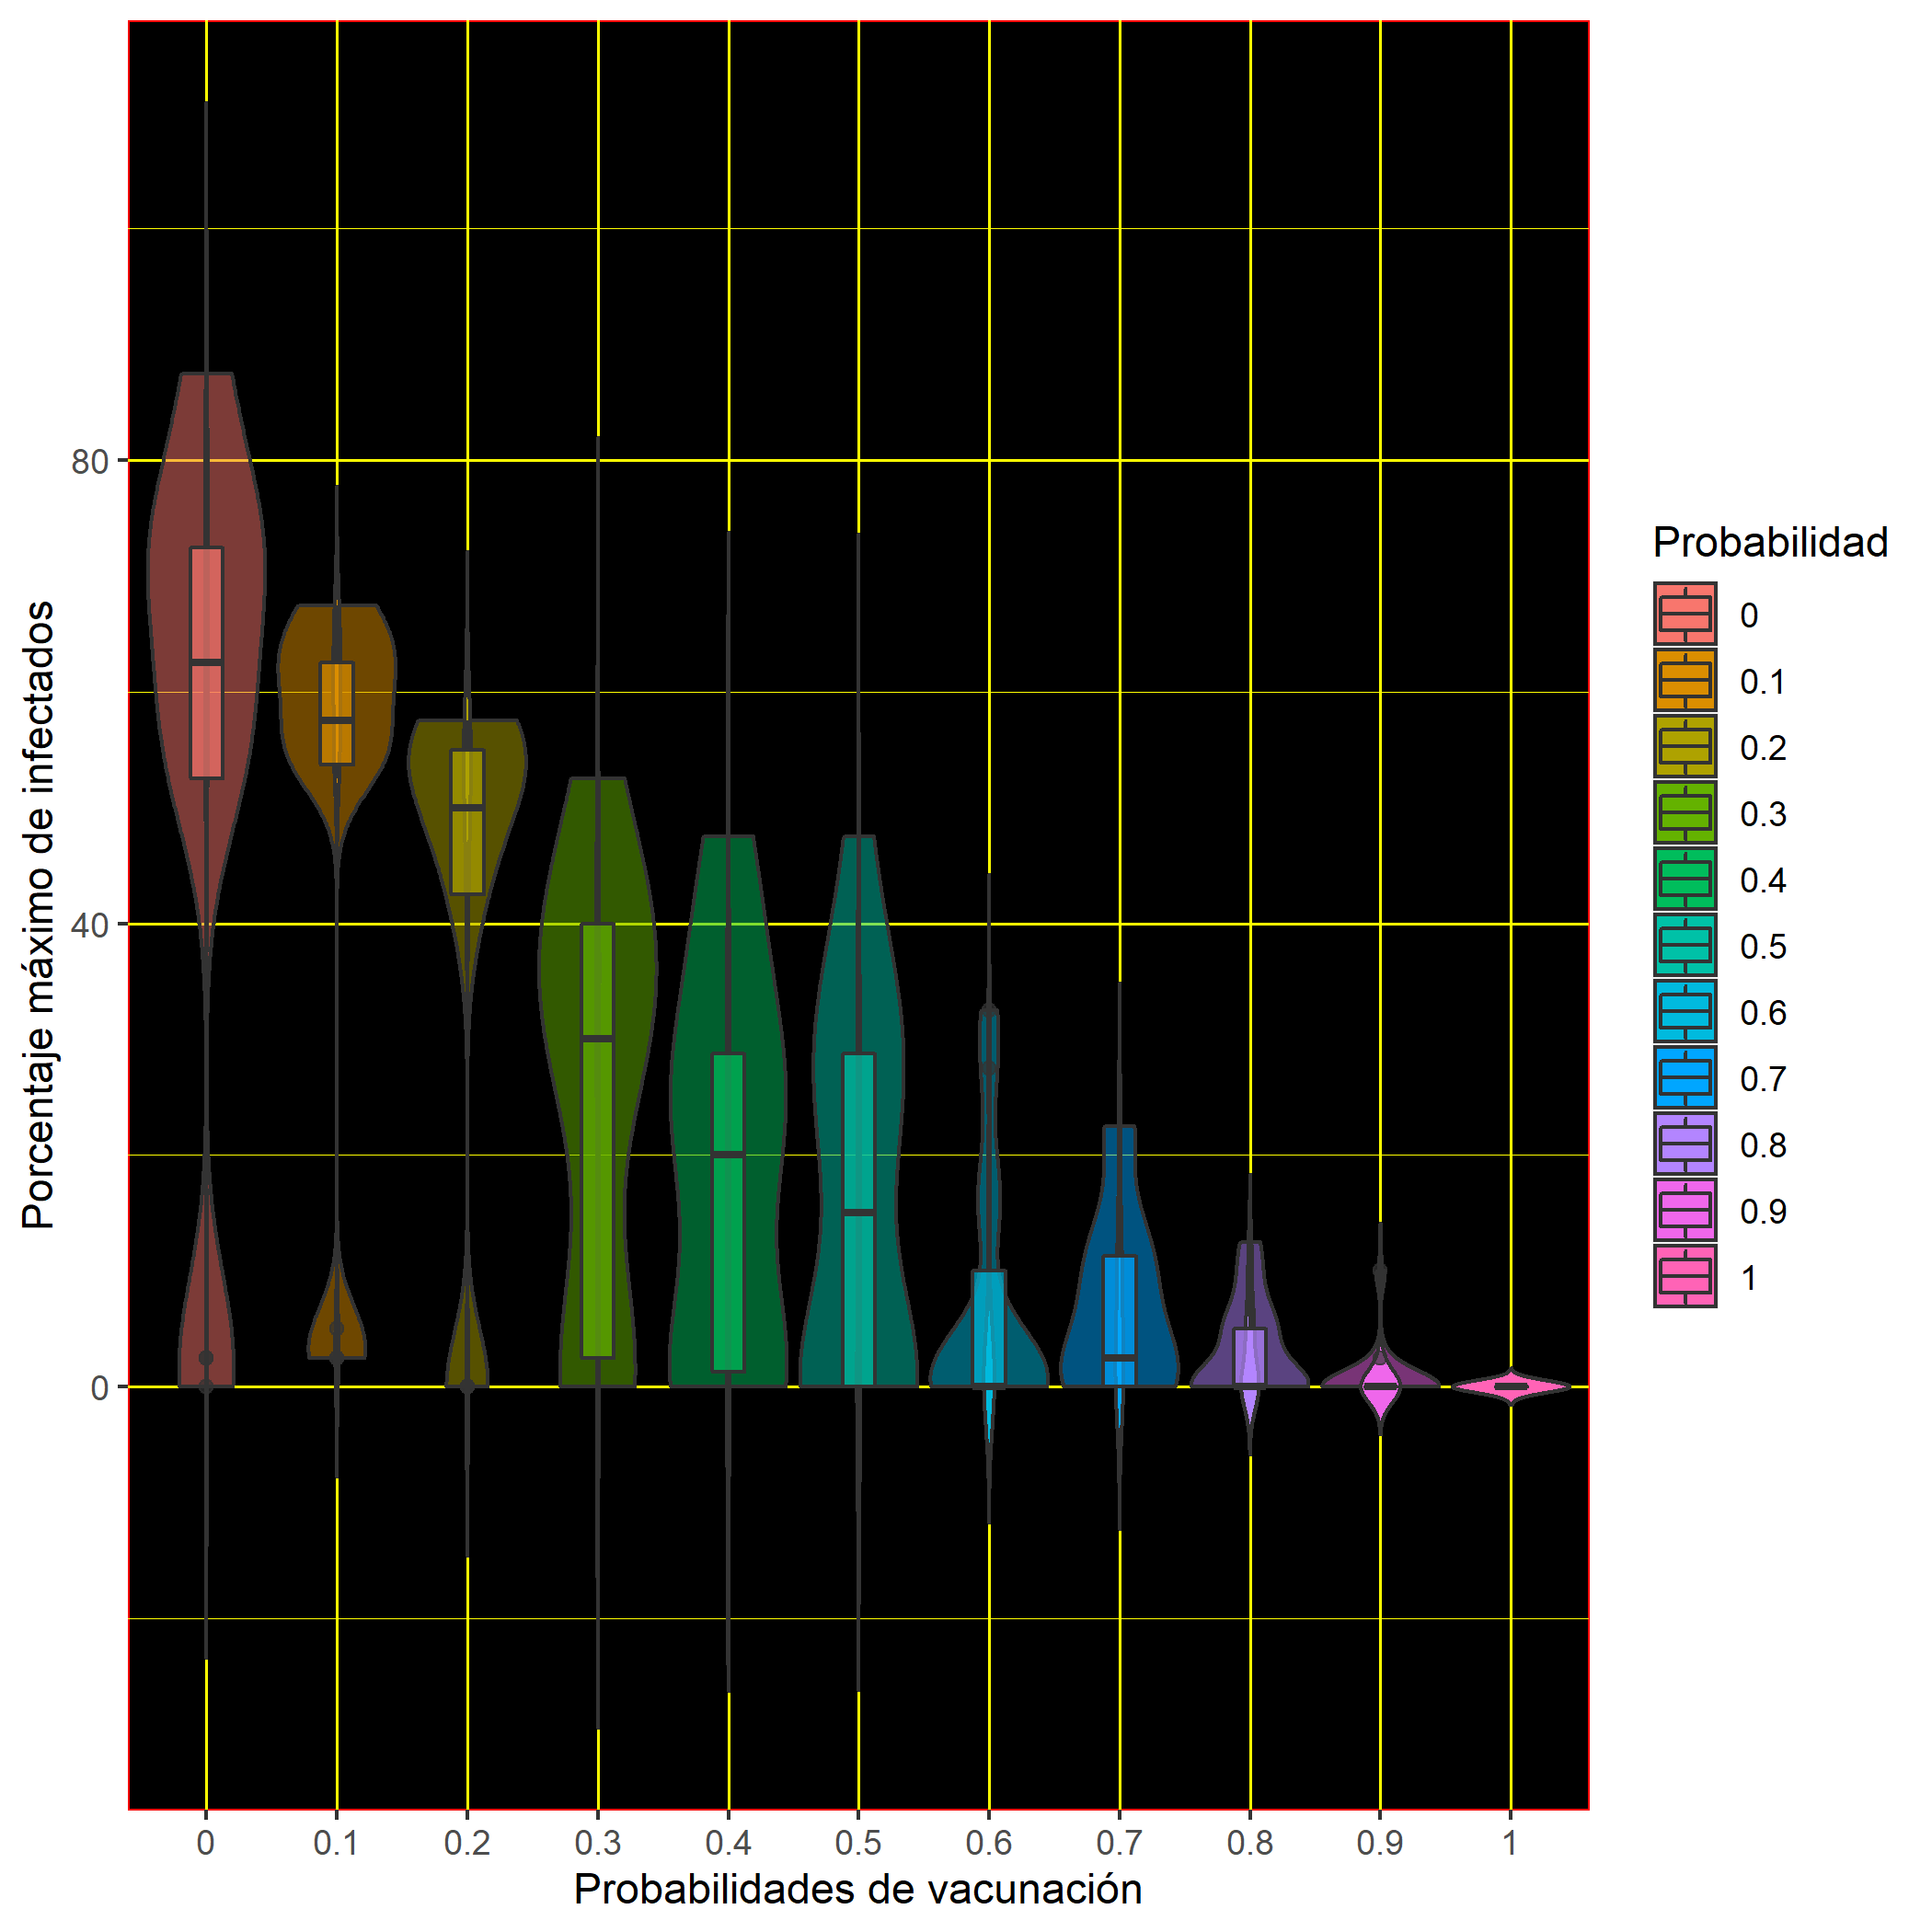
\includegraphics[scale=0.7]{Tareaseisvacunas.png}
  \caption{Porcentaje m\'aximo de contagio.}
  \label{fig}
\end{figure}

\begin{table}[H]
\centering
\caption{M\'aximos infectados respecto a la probabilidad de vacunaci\'on}
\begin{tabular}{rrrr}
\hline
Repetici\'on & Probabilidad &  Max Infectados & Porcentaje \\
\hline
9 & 0 & 35 & 87.5\%\\
29 & 0.1 & 27 & 67.5\%\\
38 & 0.2 & 23 & 57.5\%\\
46 & 0.3 & 21 & 52.5\%\\
64 & 0.4 & 19 & 47.5\%\\
76 & 0.5 & 19 & 47.5\%\\
98 & 0.6 & 13 & 32.5\%\\
113& 0.7 & 9 & 22.5\%\\
130 & 0.8 & 5 & 12.5\%\\
148 & 0.9 & 4 & 10\%\\
151 & 1 & 0 & 0\%\\

\hline
\end{tabular}
\label{t1}
\end{table}

\section{Conclusi\'on}

Despu\'es de haber realizado la simulaci\'on se muestra en ambas graficas que la disminuci\'on en el ritmo de contagio depende de la previa vacunaci\'on de los agentes pues de esta manera se evita tanto el contagio como la propagaci\'on por parte de un agente hacia el resto de la muestra; debido a que as\'i no arriesga a todos los que pueden ser vulnerables.

\bibliography{tareaseis}
\bibliographystyle{unsrtnat}

\end{document}
